\section{Statement of Problem}
Task 2 utilizes a wave ray tracing algorithm and local bathymetry information, provided for Narragansett Bay, in order to propagate storm waves determined from task 1. In order to complete this task, simulations are conducted for the 20 and 50 year storms along with creating rays that intersect along the shoreline of Narragansett Beach. For the 20 year storm simulations, use the ray spacing on the beach to calculate a refraction coefficient for each section of beach. Then, using bathymetry data from a chart near the beach, estimate the beach slope. This is used along with the deep water wave properties and refraction coefficient to estimate the shoaling coefficient, breaking depth, and breaker height. 
\section{Hypotheses and Theories}

Wave propagation from deep to shallow water is influenced by changes in the sea floor. As regions of the sea floor change with height the waves refract, and their local angle of incidence shifts. 

\section{Solution of the Problem}

\begin{figure}[H]
\centering
\includegraphics[width=1.0\textwidth]{./img/20y_150deg_hires.eps}
\caption{Wave Ray 20y Expected Wave Parameters at 150 deg Hires}
\label{fig:prob4WHvWD}
\end{figure}

\begin{figure}[H]
\centering
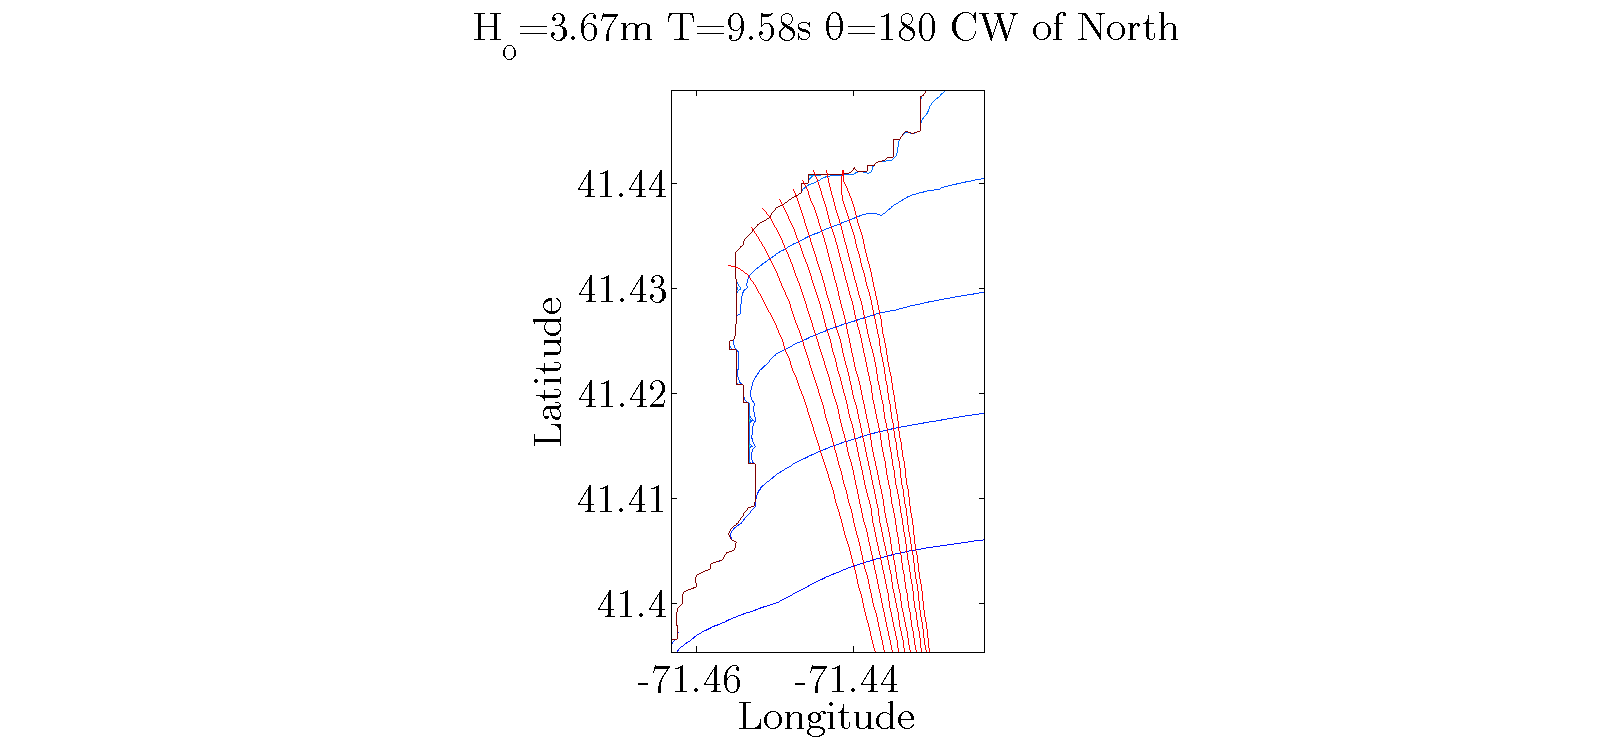
\includegraphics[width=1.0\textwidth]{./img/20y_180deg.eps}
\caption{Wave Ray 20y Expected Wave Parameters at 180 deg}
\label{fig:prob4WHvWD}
\end{figure}

\begin{figure}[H]
\centering
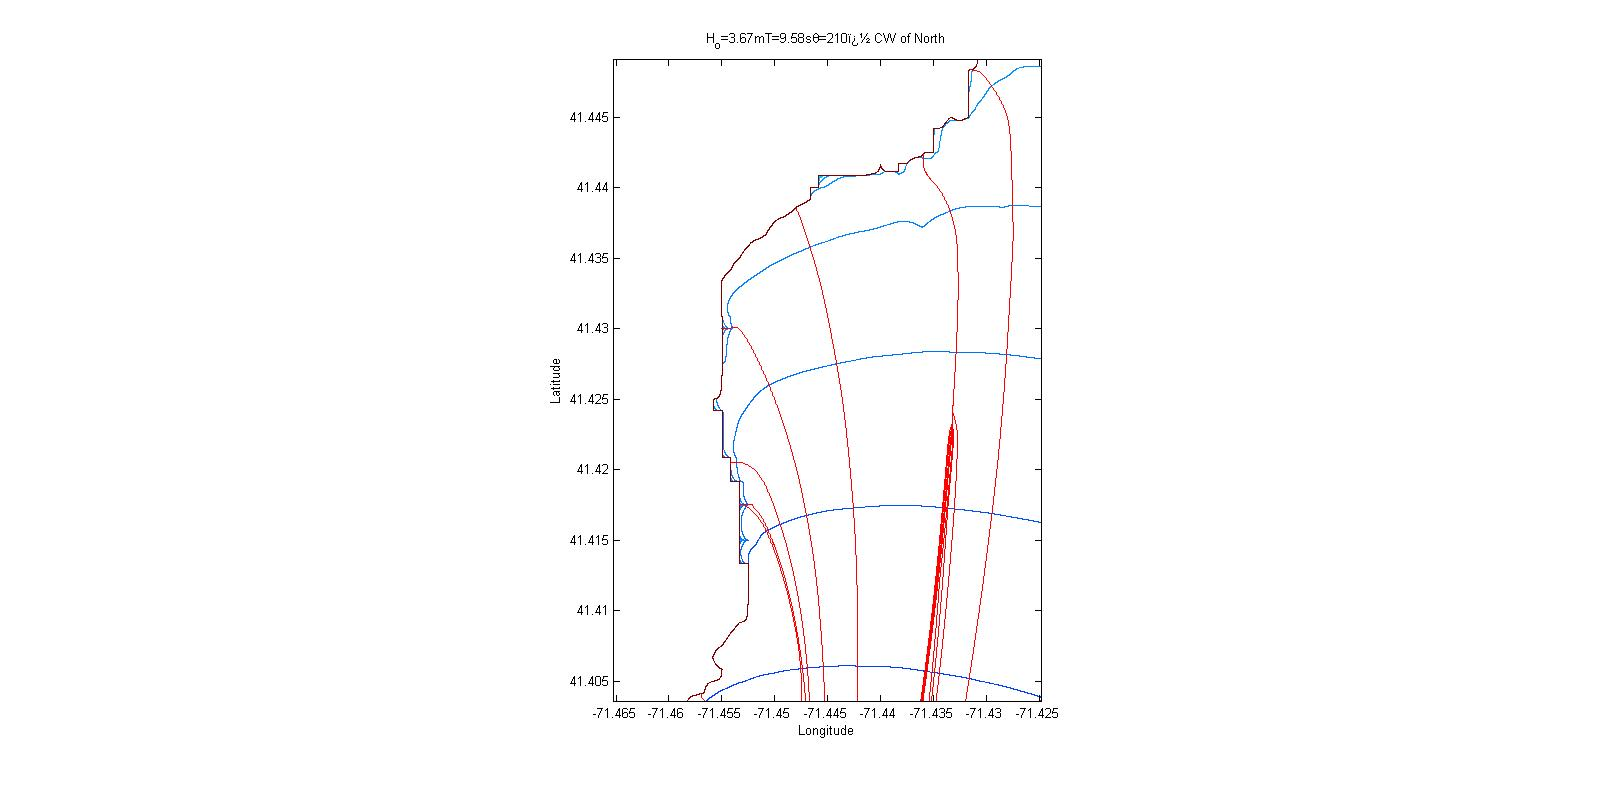
\includegraphics[width=1.0\textwidth]{./img/20y_210deg.eps}
\caption{Wave Ray 20y Expected Wave Parameters at 210 deg}
\label{fig:prob4WHvWD}
\end{figure}


\begin{figure}[H]
\centering
\includegraphics[width=1.0\textwidth]{./img/50y_150deg_hires.eps}
\caption{Wave Ray 50y Expected Wave Parameters at 150 deg}
\label{fig:prob4WHvWD}
\end{figure}

\begin{figure}[H]
\centering
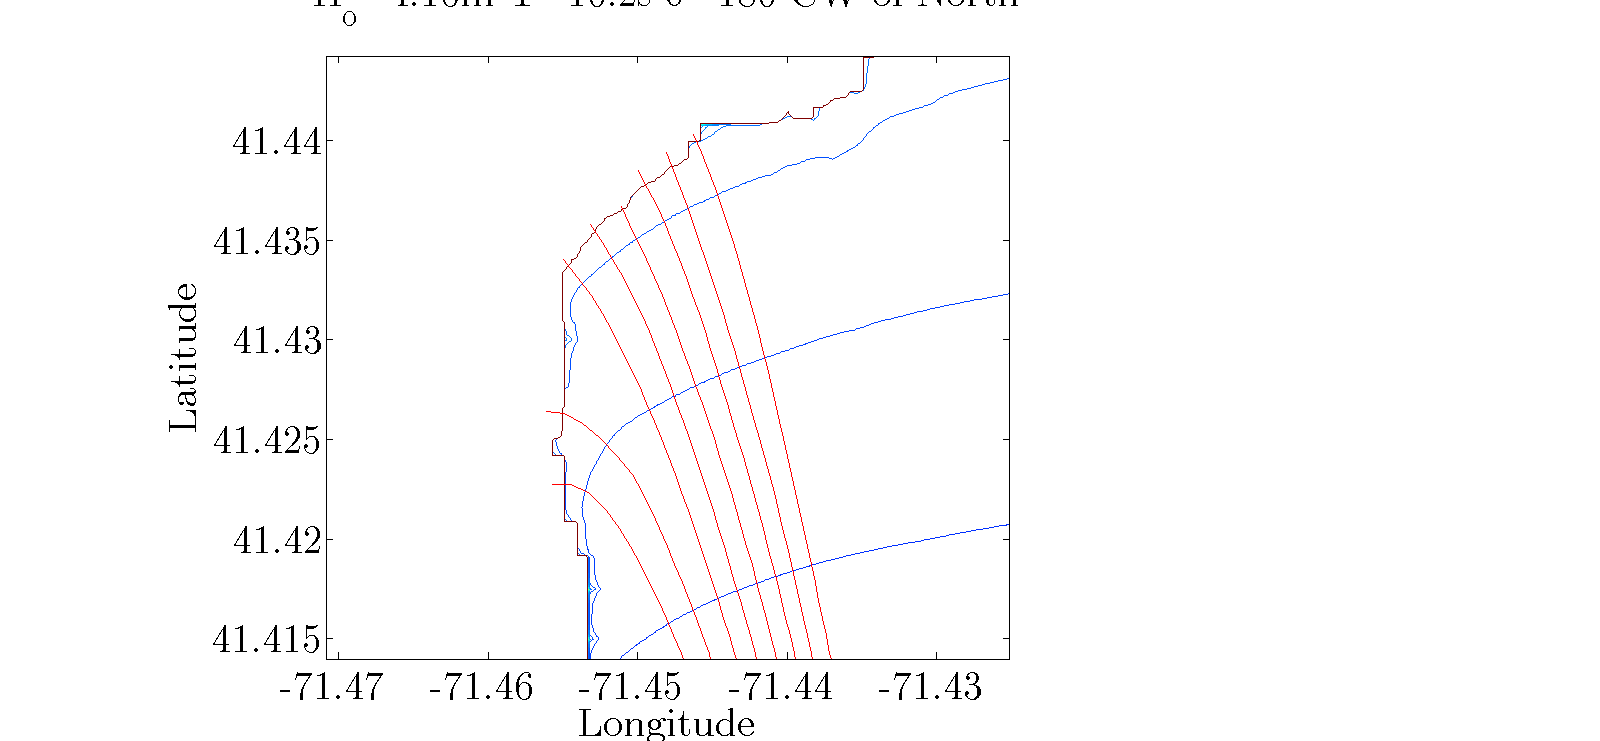
\includegraphics[width=1.0\textwidth]{./img/50y_180deg.eps}
\caption{Wave Ray 50y Expected Wave Parameters at 180 deg}
\label{fig:prob4WHvWD}
\end{figure}

\begin{figure}[H]
\centering
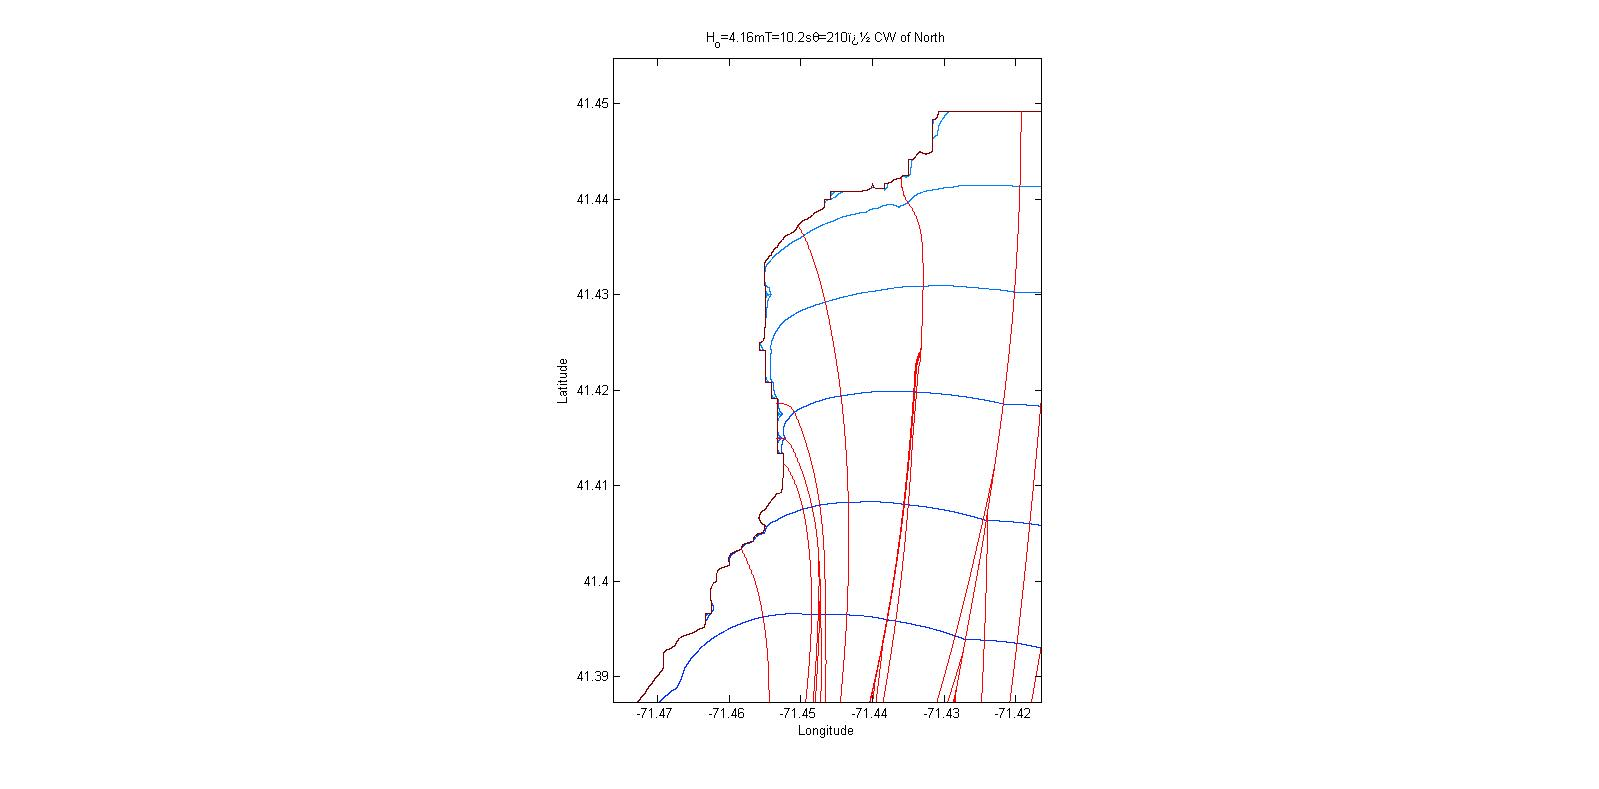
\includegraphics[width=1.0\textwidth]{./img/50y_210deg.eps}
\caption{Wave Ray 50y Expected Wave Parameters at 210 deg}
\label{fig:prob4WHvWD}
\end{figure}

\section{Conclusion}